\documentclass{article}
\usepackage[utf8]{inputenc}
\usepackage{enumitem}
\setlist{leftmargin=5.5mm}
\usepackage{graphicx}
\usepackage{grffile} 
\graphicspath{ {./images/} }
\title{SystemHW1}
\author{Sezer Demir }
\date{March 2021}


\begin{document}

\maketitle
\section{Requirements}

\setlength{\parindent}{8ex}
\hspace{\parindent} For this homework I achieved all the requirements those are mentioned in homework pdf file. I didn't use any library functions except malloc, calloc, and free. There is no warning that comes from -Wall flag or memory leak showed by valgrind including CTRL-C interruption signal. \par
\section{Design Decisions}

\begin{enumerate}[label=\alph*.), leftmargin=1.5\parindent]
  \item To print all the files those are found by the program I needed to store their associated full-path alongside their file names, depth, and types. 
  Therefore I used a linked list to achieve that. Each node stores their names, types, paths, and depths. Depth indicates how many times program must
  have opened directory to reach the found file.
  \item I used another linked list structure to store all the pointers ,those are dynamically allocated, because in case of user interrupt the program
  by pressing CTRL-C.I should have to return all the resources back.To achieve that each node, that named as clean(another structure), stores those pointers, allocated throughout the program, in a void pointer. So I could release them if a interruption signal comes. When interruption signal comes I free all the clean nodes, so with that I release all the resources.
  \item I also checked arguments to make sure that they're entered in a proper form. If user types any invalid argument program gives a warning message and terminates itself. Some argument rules are following:
  \begin{enumerate}[label =\arabic*), leftmargin=1.5\parindent]
    \item -b: takes just positive numbers (Example: 123123 valid, -123123 or 959awf569 invalid).
    \item -l: takes just positive numbers (Example: 123123 valid, -123123 or 959awf569 invalid).
    \item -f: file names cannot include '/' character in UNIX, except that character you can use any character.
    \item -t: can take only one of the 'd', 's', 'b', 'c', 'f', 'p', 'l' characters.
    \item -w: you can enter any character for that one, if there is not such a directory it prints a warning message and terminates the program.
  \end{enumerate}
\end{enumerate}

\section{Algorithm}
\hspace{\parindent} \textbf{Finding Files}

\begin{enumerate}[leftmargin=1.7\parindent]
  \item Open next file.
  \item Check all the file conditions those are provided by user with flags. 
  \item If current file satisfies all the conditions create a new node and fill all necessary information in it like file name, path, type, and depth.
  \item Repeat that process until traverse all the files under the directory that is provided by user.
\end{enumerate}

\setlength{\parindent}{5ex}
\hspace{\parindent}\textbf{Printing Founded Files}

\hspace{\parindent} To print all the files in a proper form it checkes nodes, those have information about found files, one by one. Of course, it starts checking directories from the base directory, that provided by user, to found file's directory. To achieve that it parses directory names of found file's path. And it prints sub directory name and whenever it prints a directory name, I just store it's name in a linked list and whenever I need to print another directory, first I check that the directory printed before or not by checking that linked list, that stores all the printed directory names. Therefore it could avoid print a directory name more than once. Whenever a directory name is printed, I checked that there is any found file at same directory that I parsed. If there is it prints it too. At the end it prints the found file name and repeat all those steps until all found files in linked list are printed. The sign before the names of the files is created according to their depth information. \par
\hspace{\parindent} Lets say user wanted to find a file under "/home/user/Downloads" directory. And one of the files is under              "/home/user/Downloads/sss/ddd/" path. At first iteration it parses the "sss" directory name, print it, and checks all the other found files those have "/home/user/Downloads/sss/" path and prints them too. Then adds "sss" name and it's depth as 1 (since it is right under Downloads directory. Depth is 2 for ddd for example.) to a linked list to mark it as printed directory. At the same time it marks all the found files by assigning their "found" variable to 1, so it can check whenever a directory or file will be printed before or not. After that, it parses "ddd" and so on. And repeats those processes for all found files. \par

\newpage
\section{Input and Output Examples}

\begin{figure}[!htb]
    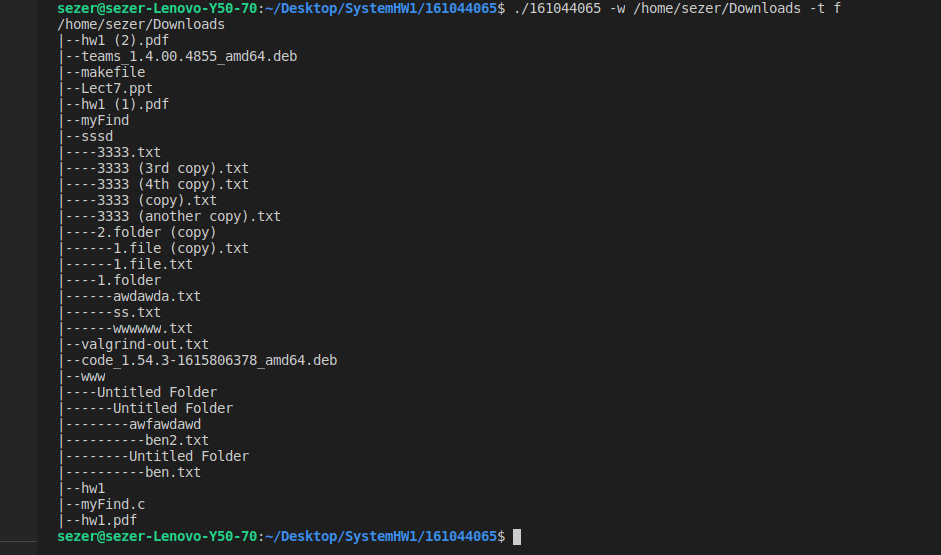
\includegraphics[scale = 0.3]{./LatexImages/output1.png}
    \caption{Valid Example 1}
\end{figure}


\begin{figure}[!htb]
    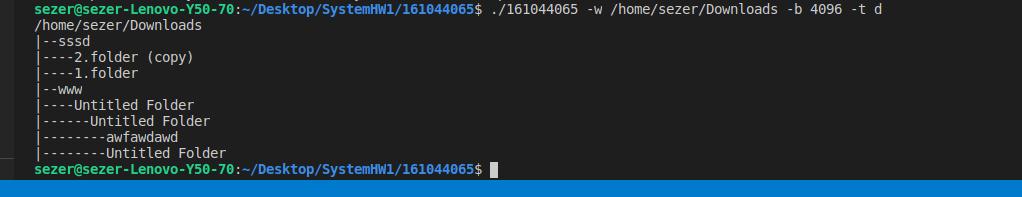
\includegraphics[scale = 0.3]{./LatexImages/output2.png}
    \caption{Valid Example 2}
\end{figure}

\begin{figure}[!htb]
    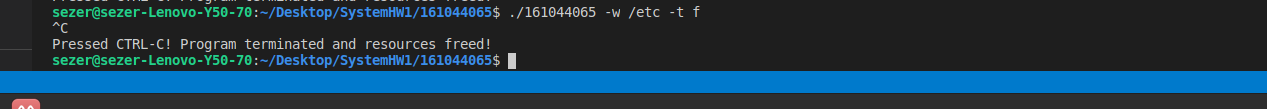
\includegraphics[scale = 0.4]{./LatexImages/output3.png}
\caption{Example of interruption by CTRL-C}
\end{figure}

\begin{figure}[!htb]
    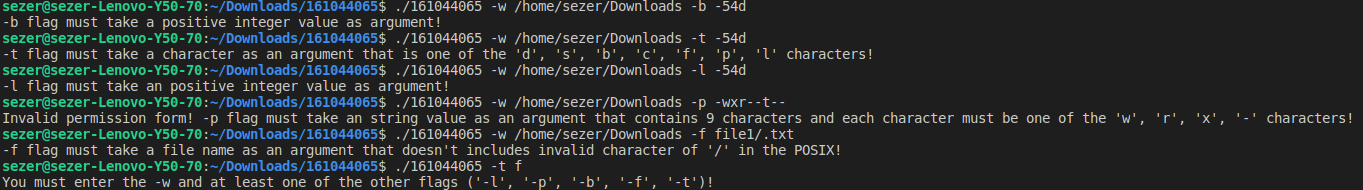
\includegraphics[scale = 0.4]{./LatexImages/output4.png}
\caption{Case of wrong entered arguments}
\end{figure}

\hspace{\parindent}\textbf{Note:That tex file compiled with pdfLaTeX compiler. Regular LaTeX compiler doesn't recognize some of the functions.} \par


\end{document}




